%-------------------------------------------------------------------------------
%-------------------------------------------------------------------------------
\section{Network inference: a brief introduction}
%-------------------------------------------------------------------------------
%-------------------------------------------------------------------------------

%-------------------------------------------------------------------------------
%-------------------------------------------------------------------------------
\subsection{Network inference}
%-------------------------------------------------------------------------------

%------------------------------------------------------------------------------
\frame{ \frametitle{Network inference}

  \paragraph{A typical situation.} Consider
  \begin{itemize}
    \item $p$ genes ($1 \leq j \leq p$)
    \item $n$ samples ($1 \leq i \leq n$)
    \item $X_{ij} =$ expression level of gene $j$ in sample $i$
  \end{itemize}

  \bigskip \pause
  \paragraph{Typical assumptions.} 
  \begin{itemize}
    \item The $n$ samples have been collected independently
    \item The vector of expressions
    $$
    X_i = [X_{i1} \dots X_{ij} \dots X_{ip}]
    $$ 
    all arise from the same (probabilistic) distribution in each sample
  \end{itemize}
  
  \bigskip
  In statistical terms: 
  $$
  \{X_i\}_{1 \leq i \leq n} \text{ iid } \sim p.
  $$
  
}

%------------------------------------------------------------------------------
\frame{ \frametitle{Network inference}

  \paragraph{Intuition.}
  \begin{itemize}
   \item The expression of a given gene in a given sample is {\sl not independent} from the expressions of all the others genes in the same sample \\
   (otherwise, the notion of 'network' vanishes) \\ ~
   \item \pause The coordinates of an expression vector $X_i$ should not independent \\ ~
   \item \pause If the network exists, is must be hidden in the joint distribution $p$.
  \end{itemize}
  
  \bigskip \bigskip \pause
  \paragraph{A mathematical definition for 'interaction':} 'gene 1 and gene 2 interact'
  $$
  \Leftrightarrow \quad 
  \text{$X_1$ and $X_2$ are {\sl dependent} conditionally on $X_3, X_4, \dots X_p$} 
  $$
}

%-------------------------------------------------------------------------------
%-------------------------------------------------------------------------------
\subsection{Graphical models}
%-------------------------------------------------------------------------------

%------------------------------------------------------------------------------
\frame{ \frametitle{Graphical models  \refer{Lau96}}

  \paragraph{(Undirected) graphical model.} The distribution $p(U) = p(U_{1}, \dots, U_m)$ is faithful to the graph $G$ iff
  $$
  j \sim k 
  \qquad \Leftrightarrow \qquad 
  (U_j, U_k) \text{ are dependent conditionally on } \{U_\ell\}_{\ell \neq j, k}
  $$

  \pause\vspace{.1\textheight}
  \begin{tabular}{cc}
    \begin{tabular}{p{.35\textwidth}}
	 \begin{tikzpicture}
\node[observed] (U3) at (0*\edgeunit, 0*\edgeunit) {$U_3$};
\node[observed] (U1) at (-0.65*\edgeunit, 1.3*\edgeunit) {$U_1$};
\node[observed] (U2) at (.65*\edgeunit, 1.3*\edgeunit) {$U_2$};
\node[observed] (U4) at (1.5*\edgeunit, 0*\edgeunit) {$U_4$};
\draw[edge] (U1) to (U2); \draw[edge] (U1) to (U3); \draw[edge] (U2) to (U3); \draw[edge] (U3) to (U4);
\end{tikzpicture}


    \end{tabular}
    & 
    \begin{tabular}{p{.55\textwidth}}
	 \begin{itemize}
	 \item Connected graph: $(U_1, U_2, U_3, U_4)$ are all dependent \\~
	 \item $(U_1, U_2)$ are dependent conditionnally on $(U_3, U_4)$ \\~
	 \item $U_3 =$ separator: $U_4 \perp (U_1, U_2) \gv U_3$ \\~ \\~
	 \end{itemize}
    \end{tabular}
  \end{tabular} 

}

%------------------------------------------------------------------------------
\frame{ \frametitle{To summarize}

  \begin{tabular}{cc}
    \hspace{-.04\textwidth}
    \begin{tabular}{p{.4\textwidth}}
      To do this: \\ ~
      \begin{itemize}
        \item we assume that the expression vectors all arise from a distribution $p$ \\ ~
        \item which is faithful to a (undirected) graph $G$
      \end{itemize}
    \end{tabular}
    & 
    \hspace{-.05\textwidth}
    \begin{tabular}{p{.5\textwidth}}
      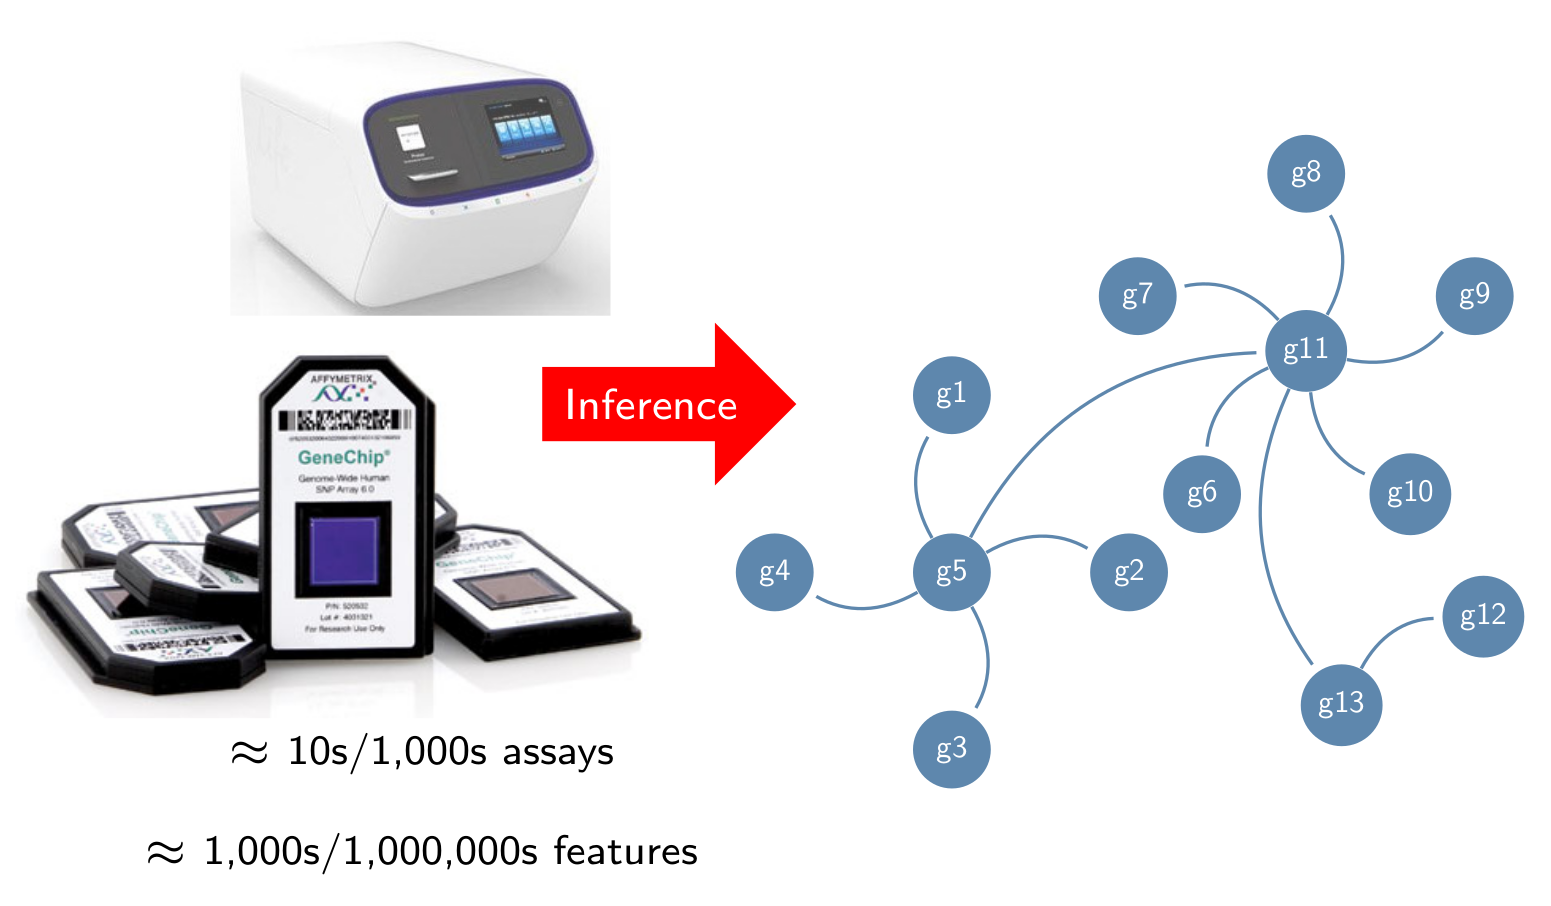
\includegraphics[width=.5\textwidth]{\fignet/Chi18-JC2BIM-p7}
    \end{tabular}
  \end{tabular}

  \bigskip \bigskip \pause
  \paragraph{Remark.}
  \begin{itemize}
    \item Directed graphical models do exist
    \item but they are often not unique ($p$ can be faithful to several directed graphs $G_1$, $G_2$, ...)
  \end{itemize}
  
}

%------------------------------------------------------------------------------
\frame{ \frametitle{Network inference}

  We want to recover $G$ ($p$ nodes, few vertices) from the data matrix $X$.
  
  \bigskip \bigskip \pause
  \paragraph{A huge task.}
  There are $\Gcal(p) = 2^{p(p-1)/2}$ possible graphs with $p$ nodes:
  $$
  \Gcal(10) = 10^{13}, \qquad \Gcal(100) = 10^{1490}, \qquad \Gcal(1000) = 10^{15364}.
  $$  
  \ra We will not try them all.
  
  \bigskip \bigskip \pause
  \paragraph{Hopefully.}
}

%-------------------------------------------------------------------------------
%-------------------------------------------------------------------------------
\subsection{Gaussian graphical models (GGM)}
%-------------------------------------------------------------------------------

%------------------------------------------------------------------------------
\frame{ \frametitle{Gaussian graphical models (GGM)}

}
%------------------------------------------------------------------------------
\frame{ \frametitle{Time course data}

}

